\subsubsection{الگوی \lr{ROOM}}
\label{archROOMSec}
\begin{RTL}
\lr{ROOM} \footnote{\lr{Real-time Object Oriented Methodology}}
\cite{ref4} یک روش قدیمی‌تر است که پیش از \lr{UML} وجود داشته است، با این حال
\lr{UML} می‌تواند \lr{ROOM} را مدل‌سازی کند، همان‌طور که توسط تطابق
\lr{UML-RT} نشان داده شده است.
\lr{ROOM} نقش‌های خاصی برای رابط‌های دوطرفه به نام پورت‌ها شناسایی می‌کند
و از کلاس‌های پروتکل برای کنترل این تعاملات استفاده می‌کند و کپسوله‌سازی قوی ارائه می‌دهد.
این روش از نمودارهای حالت برای اجرای رفتار استفاده می‌کند و برای سیستم‌هایی
با تعاملات پیچیده بین اشیاء درشت‌دانه مناسب است، چه توزیع شده
باشند یا نه. این متدولوژی کپسول‌ها را معرفی می‌کند که می‌توانند زیرکپسول‌ها را شامل شوند
و از پورت‌های رله برای ارسال پیام استفاده کنند. با وجود مزایای آن در مدیریت
رابط‌ها و تعاملات پیچیده، ماهیت سنگین \lr{ROOM} می‌تواند روابط ساده را
پیچیده کند و باید با دقت اعمال شود تا از محدودیت بیش از حد جلوگیری شود.
\end{RTL}
\begin{figure}[h!]
\centering
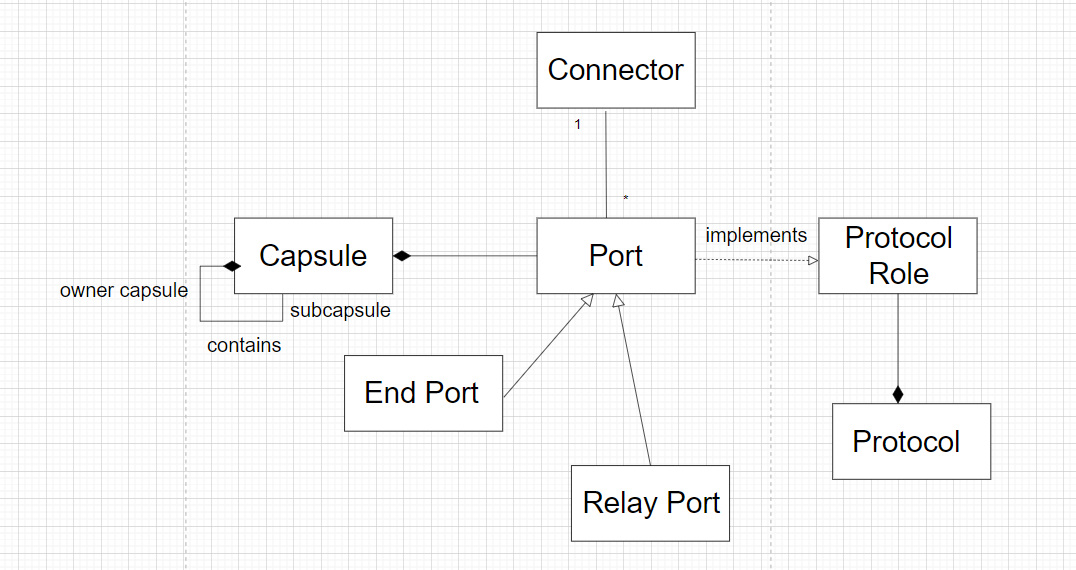
\includegraphics[scale=0.5]{images/first/room.png}
\caption{ساختار الگوی \lr{ROOM}}
\end{figure}